\section*{A: Ping Sweeping}
Ping sweep using angry IP of my home network.\\
\begin{figure}[H]
    \centering
    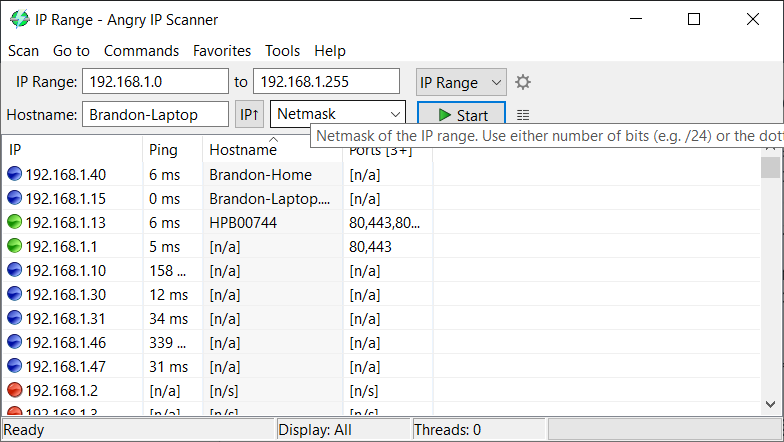
\includegraphics[width=\linewidth]{figures/a1.png}
    \caption{Angry IP output.}
\end{figure}
The output of Angry IP shows that the devices connected to the network that respond to pings and if some specified ports are opened.

\section*{B: Port Scanning}
Using the Zenmap tool I scanned Florida Poly's IP address using \verb|SYN| scan, \verb|NULL| scan, \verb|XMAS| scan and a Connection scan.

\begin{figure}[H]
    \centering
    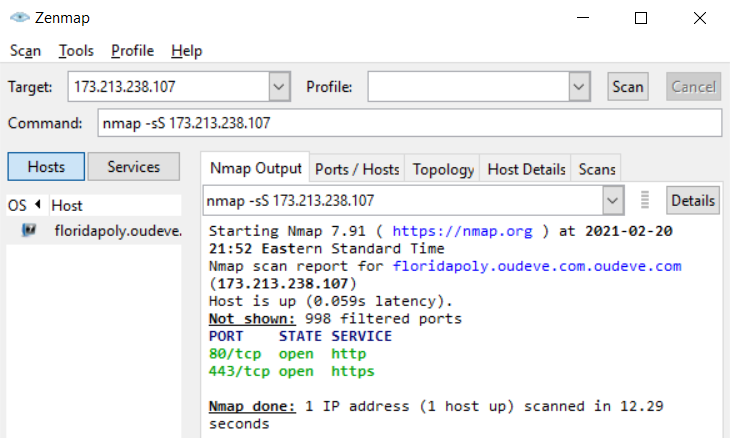
\includegraphics[width=\linewidth]{figures/b1.png}
    \caption{Zenmap output of SYN scan.}
\end{figure}
Half connect scan shows open ports via TCP but does not send the final ACK packet.
This scan tends to be faster and is less likely to be logged than the full connection scan.

\begin{figure}[H]
    \centering
    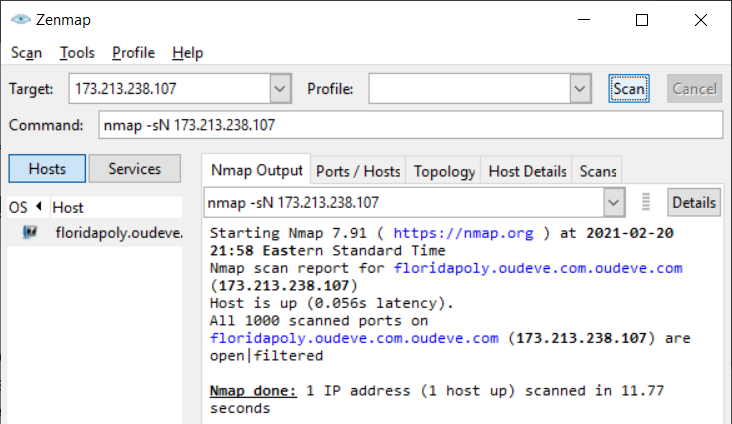
\includegraphics[width=\linewidth]{figures/b2.png}
    \caption{Zenmap output of NULL scan.}
\end{figure}
This scan sends packets with no flags enabled.
Very clearly defines if ports are opened or closed.

\begin{figure}[H]
    \centering
    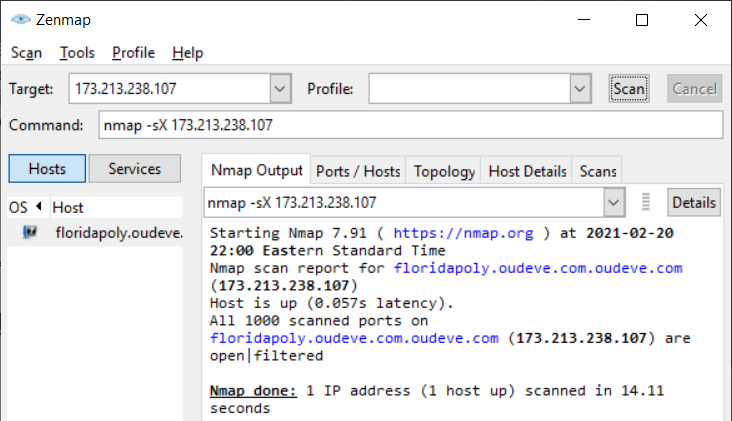
\includegraphics[width=\linewidth]{figures/b3.png}
    \caption{Zenmap output of XMAS scan.}
\end{figure}
This scan sends packets with multiple flags enabled.
If there is no response from the target it typically means that the port is open.

\begin{figure}[H]
    \centering
    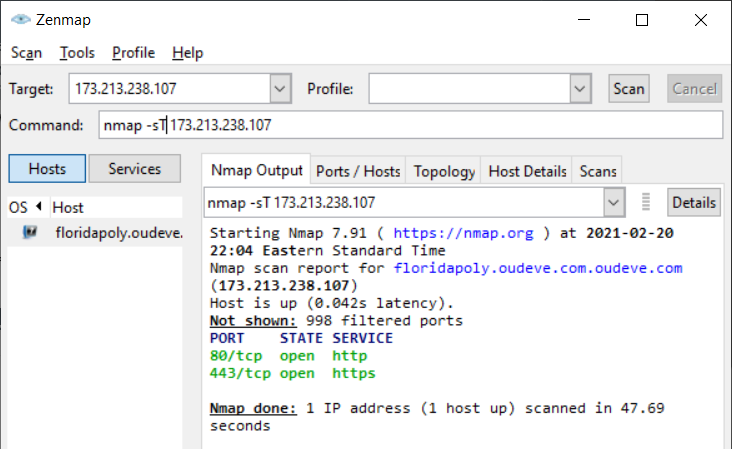
\includegraphics[width=\linewidth]{figure/b4.png}
    \caption{Zenmap output of full connect scan}
\end{figure}
The Full connect scan identifies open ports via a completed TCP handshake.
This scan is more likely to be logged.

\section*{C: Packet Crafting}
Kali Linux's \verb|hping3| tool is used to craft a packet and recieve a response from the target.
